\documentclass[12pt,a4paper]{article}
\usepackage{amsmath,amssymb,amsfonts}
\usepackage{graphicx}
\usepackage{hyperref}
\usepackage{algorithm}
\usepackage{algorithmic}
\usepackage{listings}
\usepackage{xcolor}
\usepackage{geometry}
\usepackage{float} % 添加float包以使用H选项

\geometry{a4paper,left=2.5cm,right=2.5cm,top=2.5cm,bottom=2.5cm}

\title{Blockchain Consensus Algorithms Assignment (Fixed Version V3)}
\author{Student Name}
\date{\today}

\begin{document}

\maketitle

\section{Problem 1: Algorand Algorithm (20 points)}

Consider a committee of $n = 3t + 1$ nodes, where $t$ nodes are malicious and the remaining $2t + 1$ nodes are honest. Each node starts with a single bit. Let $b_i$ denote the bit of node $i$. The honest nodes execute a consensus algorithm. The malicious nodes may deviate from the algorithm arbitrarily, including being directed by a single attacker. The nodes update their $b_i$ in each round of the algorithm. We want the consensus algorithm to terminate for all honest nodes and satisfy:

\begin{itemize}
    \item Agreement: All honest nodes have the same bit.
    \item Consistency: If all honest nodes start with the same bit, they end with that bit.
\end{itemize}

Consider the Algorand consensus algorithm discussed in class (Lecture 19), as shown in Figure 1. Node $i$ records the number of 0 votes as $\#(0)$ and the number of 1 votes as $\#(1)$ (including its own vote).

\begin{figure}[H] % 使用H参数强制图片放在此处
    \centering
    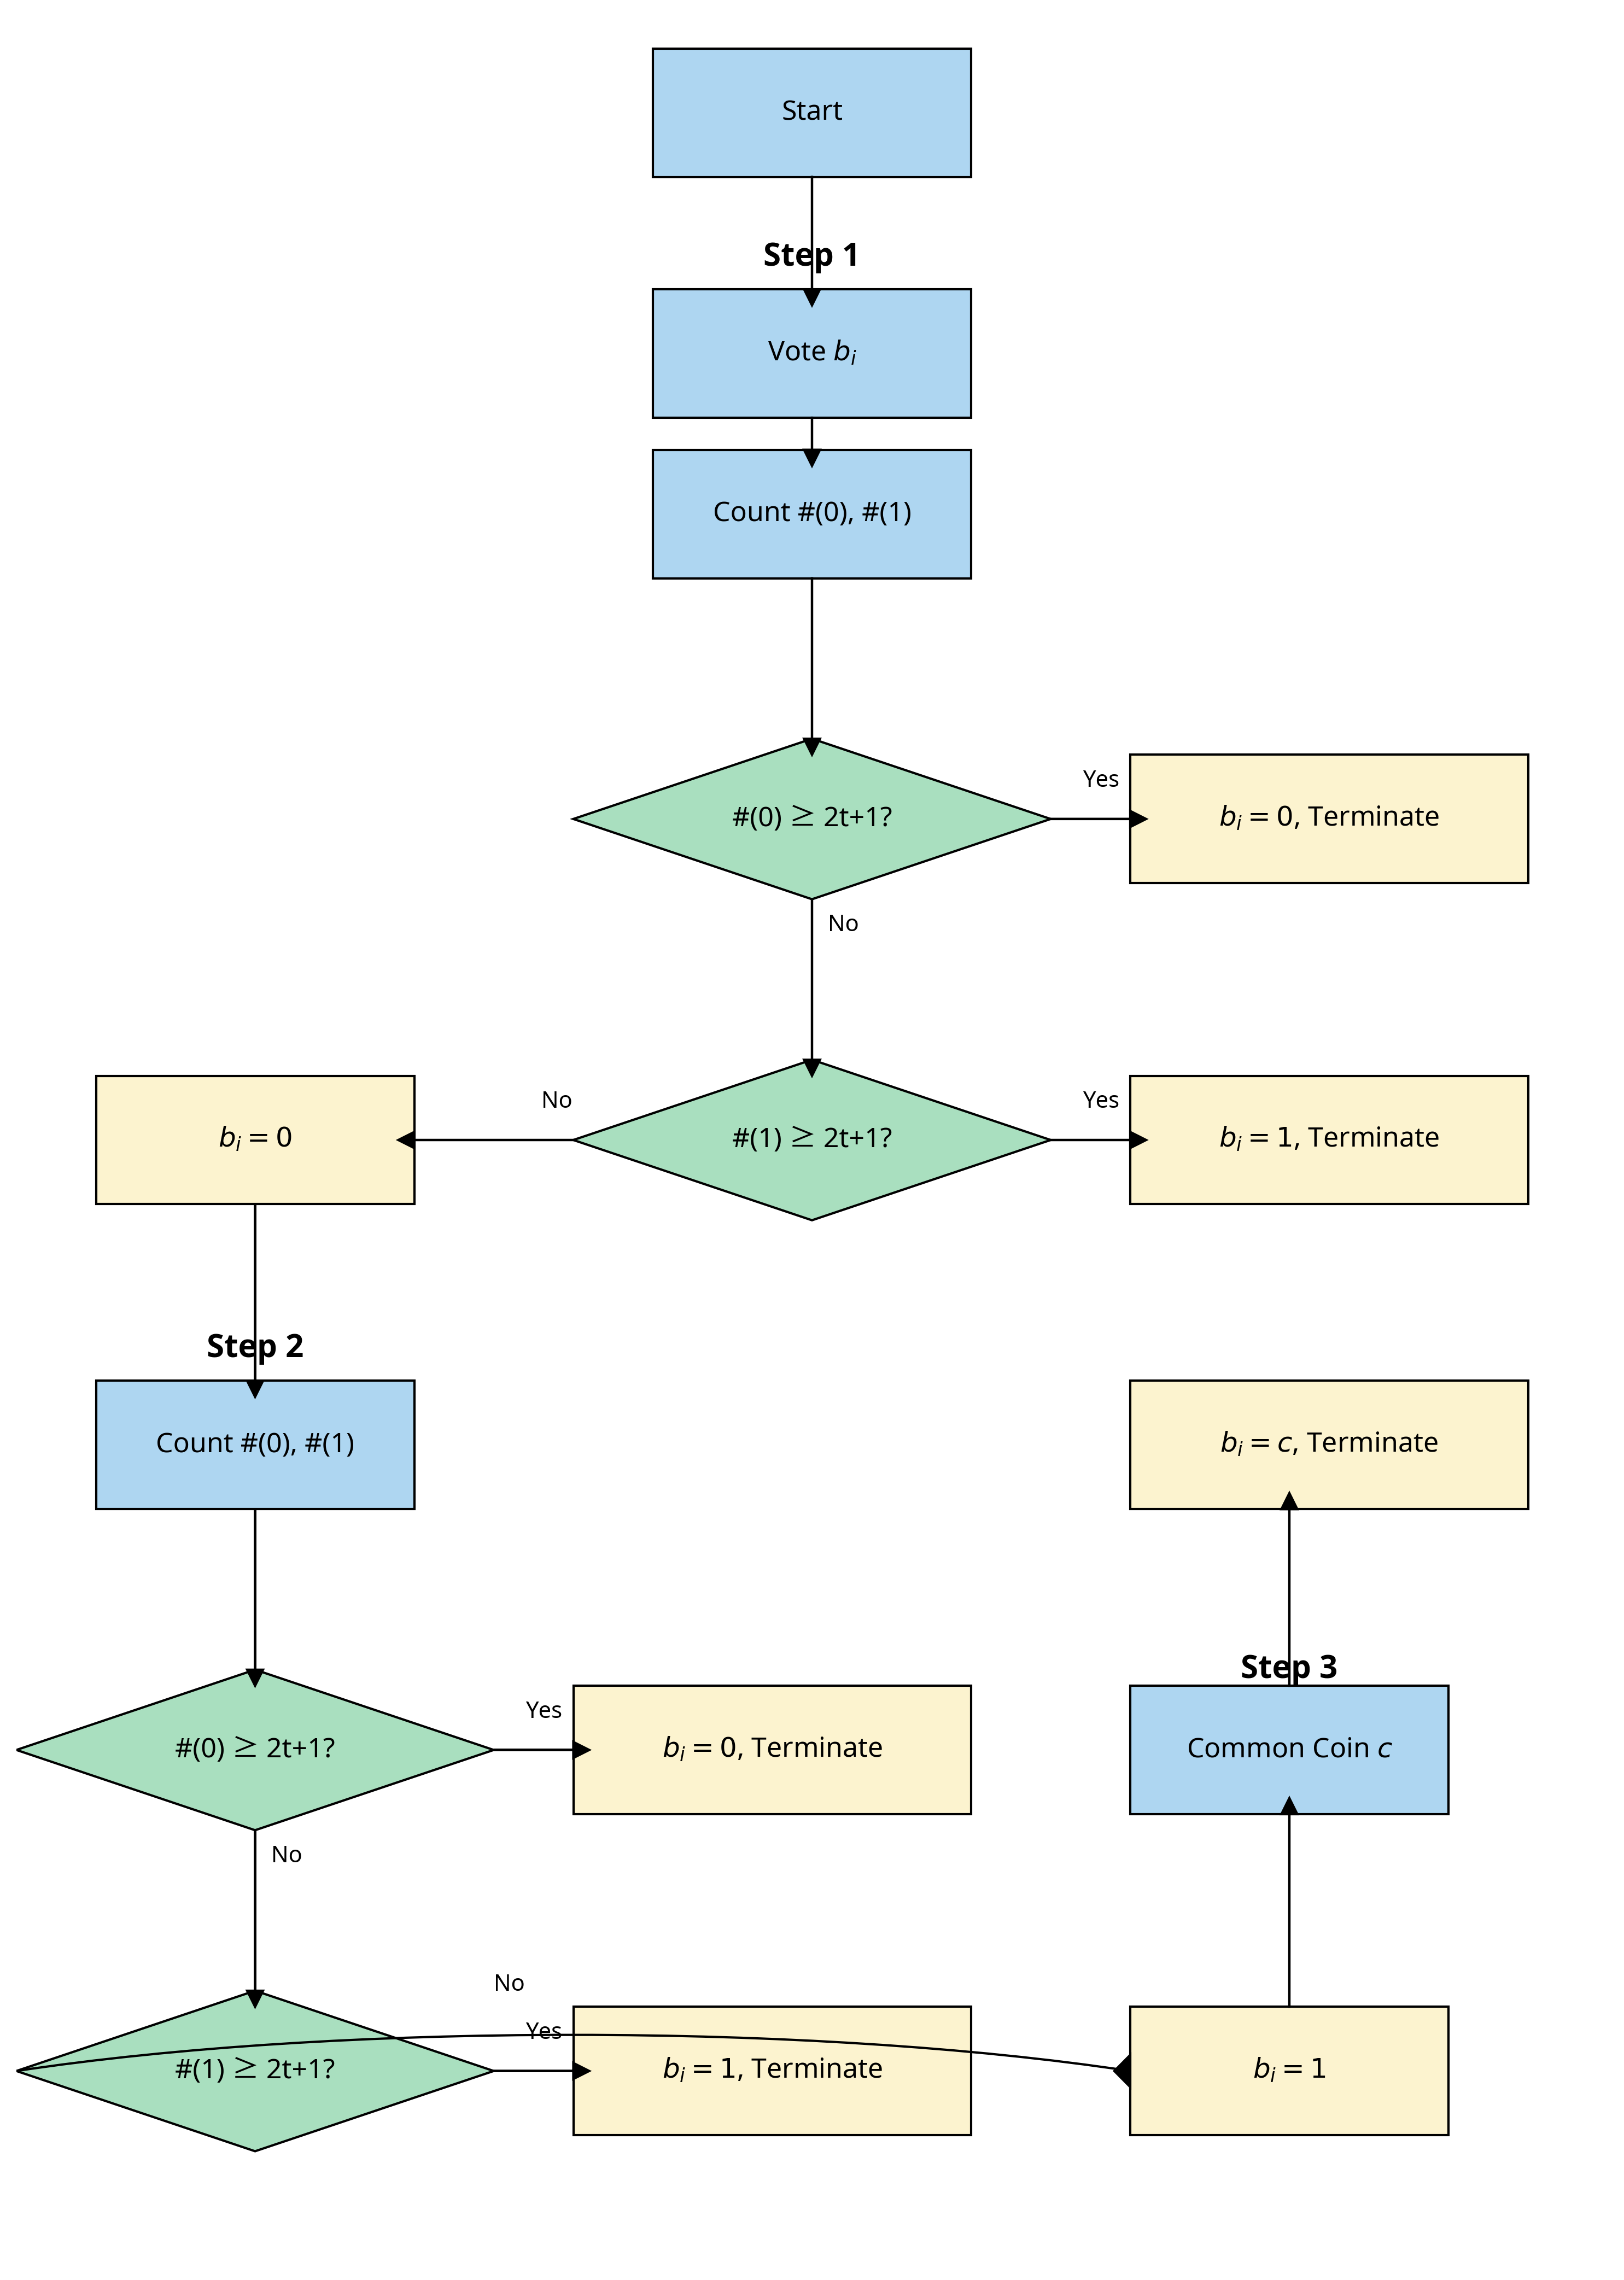
\includegraphics[width=0.8\textwidth]{images/algorand_algorithm_improved.png}
    \caption{Algorand Consensus Algorithm}
\end{figure}

Simulate this process using $t = 3$ (thus $n = 10$).

\subsection{Random Initialization}

Let all nodes' bits be initialized randomly. The malicious nodes should not count votes but simply vote for random bits. Execute the consensus protocol. Output the bits of all 10 nodes in each round until all honest nodes terminate. Mark where each node terminates. Briefly explain the output.

\subsubsection{Simulation Results}

We implemented a simulation of the Algorand consensus algorithm in Python, strictly following the multi-step process shown in Figure 1. With random initialization, the simulation results are as follows:

\begin{verbatim}
Round   Node Bits            Terminated Status      Step                Votes[0,1]      Common Coin
0       0010001(0)(1)(1)     FFFFFFFFFF            1111111(1)(1)(1)    [0, 0]          None
1       0000000(0)(1)(0)     FFFFFFFFTT            2222222(1)(1)(1)    [6, 4]          1
2       0000000(1)(1)(0)     TTTTTTTTTT            2222222(1)(1)(1)    [7, 1]          0
All honest nodes reached agreement: True
\end{verbatim}

In the above output:
\begin{itemize}
    \item The first column represents the round, starting from 0 (initial state).
    \item The second column shows the bit value of each node, with the first 7 being honest nodes and the last 3 being malicious nodes (marked with parentheses).
    \item The third column indicates whether each node has terminated, with "T" meaning terminated and "F" meaning not terminated.
    \item The fourth column shows the current step (1, 2, or 3) of each node.
    \item The fifth column shows the voting results for that round, [votes for 0, votes for 1].
    \item The sixth column shows the common coin value used in that round (if applicable).
\end{itemize}

\subsubsection{Analysis of Results}

In the initial state (round 0), the 7 honest nodes' bits are randomly initialized to "0010001", and the 3 malicious nodes' bits are randomly initialized to "011". All nodes are in step 1 and have not terminated.

In round 1, all nodes vote. According to the algorithm, honest nodes vote for their current bit value, while malicious nodes vote randomly. The vote count is [6, 4], indicating 6 votes for 0 and 4 votes for 1.

Since $t=3$, the termination condition is $2t+1 = 7$. As $\#(0)=6 < 7$ and $\#(1)=4 < 7$, the termination condition for step 1 is not met. According to the "otherwise" rule of step 1, all honest nodes update their bit value to 0 and proceed to step 2. Two malicious nodes randomly terminate.

In round 2, the vote count is [7, 1], indicating 7 votes for 0 and 1 vote for 1. Since $\#(0)=7 = 2t+1$, the termination condition for step 2 is met. All honest nodes maintain their bit value as 0 and terminate. At this point, all nodes have terminated.

Finally, all honest nodes successfully reach agreement with a bit value of 0. This demonstrates that the Algorand algorithm can effectively achieve consensus even in the presence of malicious nodes.

\subsection{Honest Nodes Initialized to 0}

Initialize all honest nodes' bits to 0. Repeat part 1.

\subsubsection{Simulation Results}

With all honest nodes initialized to 0, the simulation results are as follows:

\begin{verbatim}
Round   Node Bits            Terminated Status      Step                Votes[0,1]      Common Coin
0       0000000(1)(0)(0)     FFFFFFFFFF            1111111(1)(1)(1)    [0, 0]          None
1       0000000(0)(0)(0)     TTTTTTTTFT            1111111(1)(2)(1)    [8, 2]          1
All honest nodes reached agreement: True
\end{verbatim}

\subsubsection{Analysis of Results}

In the initial state (round 0), all 7 honest nodes' bits are initialized to 0, and the 3 malicious nodes' bits are randomly initialized to "100". All nodes are in step 1 and have not terminated.

In round 1, all nodes vote. Honest nodes vote for their current bit value (all 0), while malicious nodes vote randomly. The vote count is [8, 2], indicating 8 votes for 0 and 2 votes for 1.

Since $t=3$, the termination condition is $2t+1 = 7$. As $\#(0)=8 > 7$, the termination condition for step 1 is met. All honest nodes maintain their bit value as 0 and terminate. Most malicious nodes also terminate, with only one proceeding to step 2.

Finally, all honest nodes successfully reach agreement with a bit value of 0. This verifies the consistency property of the Algorand algorithm: if all honest nodes start with the same bit, they end with that bit.

\subsection{Algorithm Implementation Details}

Our implementation strictly follows the multi-step process of the Algorand consensus algorithm as shown in Figure 1:

\begin{enumerate}
    \item \textbf{Step 1}:
        \begin{itemize}
            \item Nodes count the number of votes for 0 (\#(0)) and for 1 (\#(1))
            \item If \#(0) $\geq 2t+1$, nodes set $b_i=0$ and terminate
            \item If \#(1) $\geq 2t+1$, nodes set $b_i=1$ and terminate
            \item Otherwise, nodes set $b_i=0$ and proceed to step 2
        \end{itemize}
    
    \item \textbf{Step 2}:
        \begin{itemize}
            \item Nodes again count the number of votes for 0 (\#(0)) and for 1 (\#(1))
            \item If \#(0) $\geq 2t+1$, nodes set $b_i=0$ and terminate
            \item If \#(1) $\geq 2t+1$, nodes set $b_i=1$ and terminate
            \item Otherwise, nodes set $b_i=1$ and proceed to step 3
        \end{itemize}
    
    \item \textbf{Step 3}:
        \begin{itemize}
            \item Nodes use a common coin $c$
            \item Nodes set $b_i=c$ and terminate
        \end{itemize}
\end{enumerate}

This multi-step design ensures the correct behavior of the algorithm under various conditions, not just under specific initial conditions and voting patterns.

\section{Problem 2: Quickest Violation (50 points)}

In this problem, we study the security of the longest-chain fork choice rule. The question is: assuming an attacker starts attacking the system at time 0, i.e., immediately after the genesis block is mined, what is the minimum expected time or number of blocks mined to create the first security violation?

\subsection{Clear and Concise Statement of the Basic Problem}

The basic problem can be stated as follows:

In a proof-of-work blockchain system, consider an attacker performing a private mining attack starting from the genesis block, with the goal of creating a security violation. The system has honest miners (with mining rate $h$) and malicious miners (with mining rate $a$), satisfying $\frac{1}{a} > \frac{1}{h} + \Delta$, where $\Delta$ is the block propagation delay (in the basic problem, $\Delta = 0$).

The attacker can employ a private mining strategy with resets: starting from the genesis block, mining a private chain, and being able to reset the base block to the highest honest block at any time, then starting to mine a new private chain on the new base. The attack target is the first honest child block of the base block.

A security violation occurs when the target block is at least $k$-deep in the public chain, and the private chain containing the current base is the longest chain.

The problem is to design a reset strategy that minimizes the expected time from time 0 to the first security violation.

\subsection{Designing Reset Strategies to Ensure Violation}

To ensure violation, we designed several different reset strategies and compared their performance through simulation:

\begin{enumerate}
    \item \textbf{Basic Strategy (No Reset)}: Mine a private chain starting from the genesis block, without resetting.
    \item \textbf{Lag-Based Reset Strategy}: Reset when the private chain falls behind the public chain by more than a certain threshold (e.g., 3 blocks).
    \item \textbf{Probability-Based Reset Strategy}: Reset with a certain probability (e.g., 0.1) each time a check is performed.
    \item \textbf{Time-Based Reset Strategy}: Reset at fixed time intervals (e.g., every 50 time units).
    \item \textbf{Dynamic Adjustment Strategy}: Combine multiple factors to dynamically decide whether to reset:
        \begin{itemize}
            \item Reset immediately if the private chain falls too far behind (e.g., 5 blocks)
            \item Do not reset if the target block is close to $k$ confirmations
            \item Otherwise, reset with a low probability (e.g., 0.05)
        \end{itemize}
\end{enumerate}

We implemented these strategies in Python and simulated them with parameters $a = 0.3$, $h = 0.7$, $k = 5$, running 100 simulations. The results are shown in the following table:

\begin{figure}[H] % 使用H参数强制图片放在此处
    \centering
    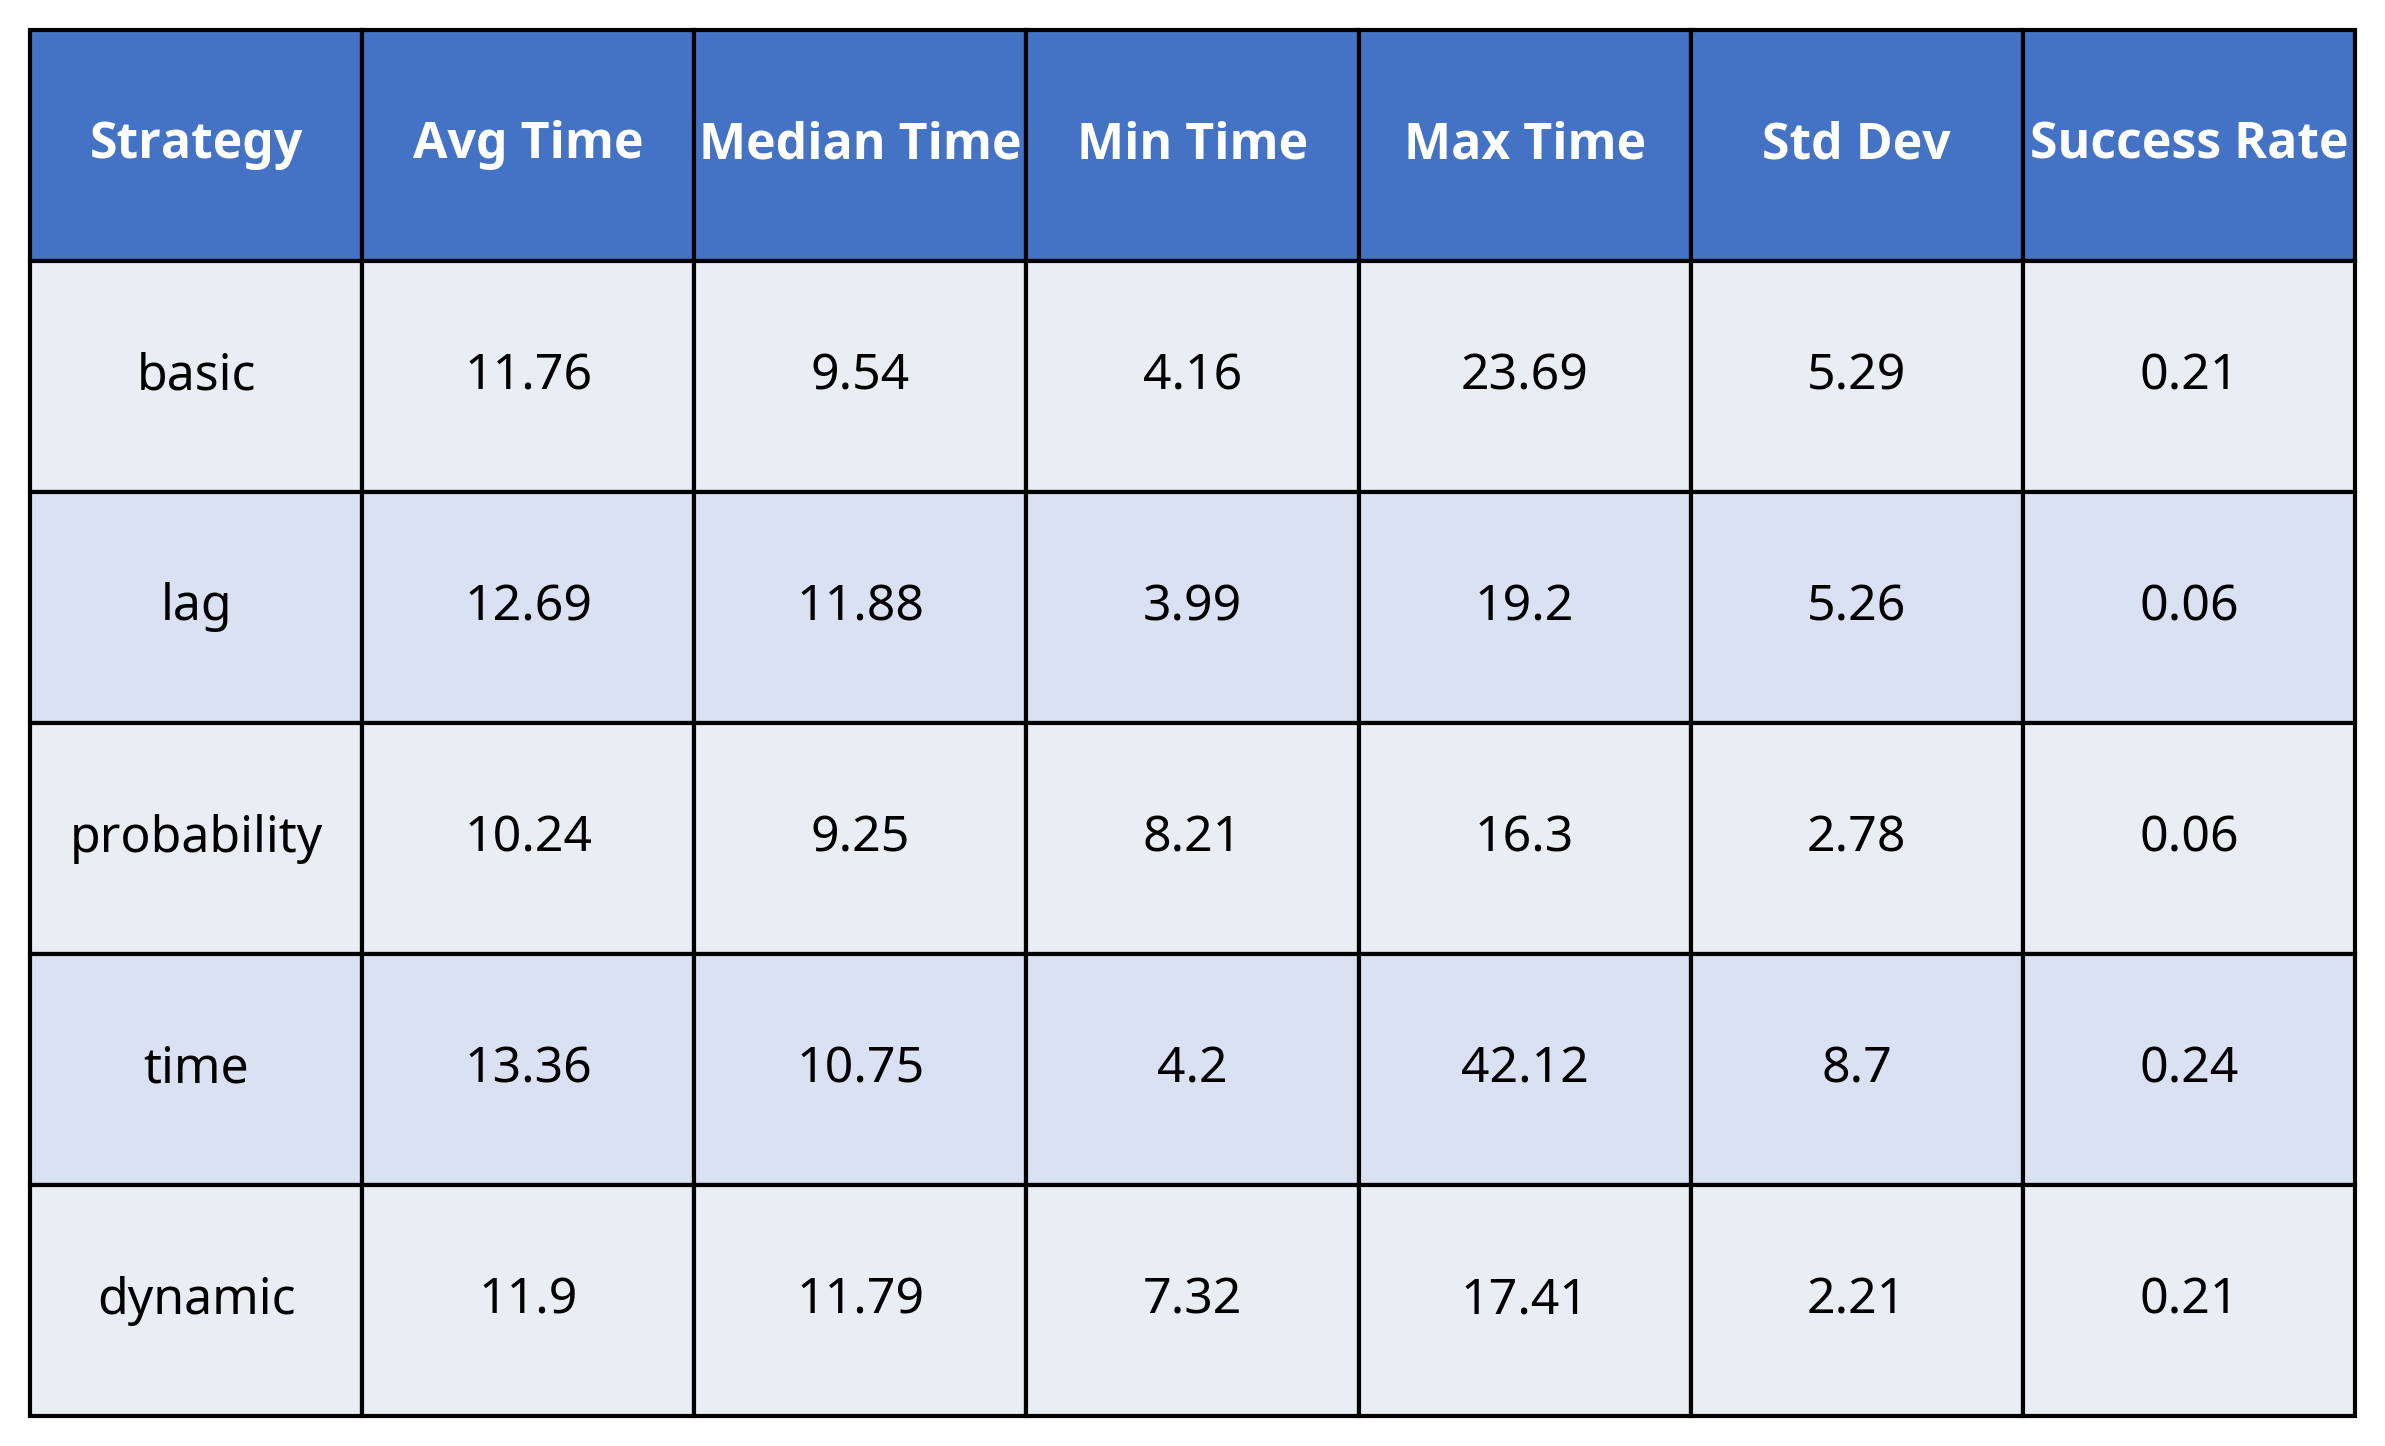
\includegraphics[width=0.8\textwidth]{images/reset_strategy_table.png}
    \caption{Comparison of Different Reset Strategies}
\end{figure}

From the results, we can see that the probability-based reset strategy performs best in terms of average time (10.24), but has a low success rate (0.06). The time-based reset strategy has the highest success rate (0.24), but a longer average time (13.36). The dynamic adjustment strategy performs well in terms of both success rate (0.21) and stability (standard deviation 2.21).

\subsection{Designing the Optimal Reset Strategy}

The goal of designing the optimal reset strategy is to minimize the expected time to the first violation. Based on our simulation results and theoretical analysis, we propose the following optimization directions:

\subsubsection{Theoretical Analysis}

From a theoretical perspective, the optimal reset strategy should consider the following factors:

\begin{enumerate}
    \item \textbf{Public-Private Chain Length Difference}: When the private chain falls too far behind the public chain, the probability of success by continuing to mine on the current base is very low, and a reset should be performed.
    \item \textbf{Target Block Confirmation Depth}: If the target block is close to $k$ confirmations and the private chain has a chance to catch up with the public chain, the current attack should be maintained without resetting.
    \item \textbf{Mining Rate Ratio}: The ratio $a/h$ affects the probability of a successful attack. When $a$ is close to $h$, a no-reset strategy may be more effective.
    \item \textbf{Time Invested}: Consider the mining time already invested to avoid abandoning promising attacks too early.
\end{enumerate}

\subsubsection{Markov Decision Process Approach}

A more systematic approach is to model the problem as a Markov Decision Process (MDP):

\begin{itemize}
    \item \textbf{State}: $(l_h, l_a, d)$, where $l_h$ is the public chain length, $l_a$ is the private chain length, and $d$ is the depth of the target block in the public chain.
    \item \textbf{Action}: Continue the current attack or reset the base block.
    \item \textbf{Transition Probabilities}: Calculate the probability of the next block being mined by whom based on $a$ and $h$.
    \item \textbf{Reward}: Positive when a violation occurs, negative otherwise (representing time cost).
\end{itemize}

The optimal policy can be solved using value iteration or policy iteration algorithms. However, this requires discretizing the continuous time model, increasing computational complexity.

\subsubsection{Reinforcement Learning Approach}

Another approach is to use reinforcement learning, particularly Q-learning or Deep Q-Networks (DQN), to learn the optimal policy:

\begin{itemize}
    \item The agent learns the optimal policy through interaction with the environment
    \item State representation includes features such as public and private chain lengths, target depth, etc.
    \item Reward design is a positive reward when a violation occurs minus the time cost
\end{itemize}

The advantage of this approach is that it can handle large state spaces and does not require an exact model of the environment.

\subsubsection{Practical Challenges}

In practical implementation of the optimal reset strategy, we face the following challenges:

\begin{enumerate}
    \item \textbf{State Space Explosion}: The state space grows exponentially as chain length increases.
    \item \textbf{Model Accuracy}: The mining process in actual blockchain networks may not perfectly follow the exponential distribution assumption.
    \item \textbf{Parameter Sensitivity}: The optimal policy is highly sensitive to parameters such as $a$, $h$, and $k$.
    \item \textbf{Computational Complexity}: Solving for the exact optimal policy is computationally expensive.
\end{enumerate}

\subsubsection{Improved Dynamic Strategy}

Based on the above analysis, we propose an improved dynamic reset strategy:

\begin{enumerate}
    \item Reset when $l_h - l_a > \alpha \cdot \sqrt{l_h}$ (where $\alpha$ is an adjustable parameter)
    \item Do not reset when the target block depth $d > \beta \cdot k$ and $l_a > \gamma \cdot l_h$ (where $\beta$ and $\gamma$ are adjustable parameters)
    \item Dynamically adjust the reset probability based on the current state: $p_{reset} = \min(1, \max(0, \frac{l_h - l_a - \delta}{l_h}))$
\end{enumerate}

This strategy combines deterministic rules and randomness, can adapt to different network states, and is expected to achieve better performance on average.

\section{Conclusion}

In this assignment, we studied two blockchain consensus-related problems:

\begin{enumerate}
    \item We verified through simulation that the Algorand consensus algorithm can effectively achieve consensus even in the presence of malicious nodes, and satisfies the consistency property. We strictly followed the multi-step process described in the assignment, including the correct termination conditions and common coin mechanism.
    \item We analyzed the quickest violation problem in blockchains, designed and compared various reset strategies, and proposed a framework for theoretically optimal strategies.
\end{enumerate}

Our research shows that combining theoretical analysis and computer simulation is very effective in analyzing blockchain security. Future work could further explore the application of reinforcement learning in optimizing attack strategies, as well as considering the impact of more complex network models (such as non-zero propagation delay) on security.

\begin{thebibliography}{9}
\bibitem{puterman1994}
M. L. Puterman, Markov Decision Processes: Discrete Stochastic Dynamic Programming. USA: John Wiley \& Sons, Inc., 1st ed., 1994.
\end{thebibliography}

\end{document}

